\chapter{Context}\label{chap2}

\section{Institutional Framework}
This six-month internship was conducted at the \textbf{Laboratoire Ville Mobilité Transport (LVMT)}, a research unit affiliated with \textbf{École nationale des ponts et chaussées (ENPC)}, with funding provided by the \textbf{Energy4Climate interdisciplinary center (E4C)}. This institutional arrangement reflects the collaborative nature of contemporary energy and mobility research to address complex challenges in sustainable transportation infrastructure. The following sections detail the structure, missions, and research orientations of these three interconnected organizations that provided the framework for this research project.

\textbf{ENPC} represents one of France's most prestigious engineering institutions. Founded in 1747 by Daniel-Charles Trudaine, ENPC is among the oldest French Grandes Écoles, historically focused on training engineering officials and civil engineers. The school has evolved to offer wide-ranging education including computer science, applied mathematics, civil engineering, mechanics, finance, economics, innovation, urban studies, environment and transport engineering. In July 2024, ENPC became the sixth member school of Institut Polytechnique de Paris (IP Paris), joining École polytechnique, ENSTA Paris, ENSAE Paris, Télécom Paris and Télécom SudParis.

Located on the Champs-sur-Marne campus, ENPC maintains a strong international presence with 43\% of its students obtaining double degrees abroad and 30\% of the engineering cohort being international students. The institution's research excellence is supported by 12 research laboratories, covering domains crucial to ecological, digital, and energy transitions, positioning it as a key player in addressing contemporary sustainability challenges.

\textbf{LVMT} serves as the direct host institution for this research project. Created in 2003, this multidisciplinary research laboratory operates as a joint research unit between Université Gustave Eiffel and École nationale des ponts et chaussées. Celebrating its 20th anniversary in 2023, LVMT brings together nearly 90 researchers in social sciences and engineering sciences, with expertise spanning economics, anthropology, sociology, geography, urban planning, technical economics, mathematical modeling, and computer science.

The laboratory's scientific objective centers on understanding and modeling interactions between mobility practices, transport infrastructure, and spatial organization and development. Research activities are organized around four thematic axes: mobility practices and urban access; territorial dynamics and public action; city-transport interactions; and economic analysis and transport modeling. LVMT researchers collaborate extensively with national and international laboratories as well as public and private transport and urban planning stakeholders, including territorial authorities, public decision-makers, ADEME, RATP, SNCF, and Transdev. This collaborative approach combines quantitative methods and qualitative analyses, positioning the laboratory at the interface between academic research and action research.

\textbf{E4C} provides the funding framework and broader research context for this internship. Launched in June 2019 by IP Paris and ENPC, E4C addresses energy transition through research, training, and innovation. The center gathers 21 laboratories from Institut Polytechnique de Paris and 5 associated laboratories from ENPC, creating a unique interdisciplinary platform for energy and climate research.

Nearly 30 laboratories work within E4C on four cross-cutting themes designed to reduce greenhouse gas emissions, improve energy efficiency, deploy renewable energy, and propose relevant energy policies. The center combines diverse scientific disciplines including social and economic sciences, materials sciences and engineering, applied mathematics, computer science, and geophysics. E4C develops instrumental platforms, models for energy forecasting and prediction, and maintains a comprehensive data center: the E4C DataHub.

The framework of this internship within E4C directly aligns with the center's mission to foster interdisciplinary collaboration addressing energy transition challenges. The digital twin development for EV charging infrastructure contributes specifically to E4C's objectives of improving energy efficiency and supporting the deployment of sustainable transportation solutions, demonstrating the practical application of interdisciplinary research in addressing real-world sustainability challenges.

\section{Research Supervision and Project Framework}

\subsection{Research Supervision Team}

This internship project was conducted under the joint supervision of two tutors, 
reflecting the interdisciplinary nature of digital twin technologies and their 
application to energy mobility systems.

\textbf{Dr. Daphné Tuncer} is my supervisor from ENPC, specializing in 
digitalisation in the energy and mobility sectors.  Prior to joining ENPC, She spent many years in the UK Higher Education. Her research keywords include electric mobility, cyberphysical systems, data management, and applied data science.

\textbf{Dr. Georgios Bouloukakis} from Télécom SudParis, provides co-supervision with expertise in IoT/Edge-driven middleware and distributed software 
systems. He is an experienced researcher and educator with over one decade of teaching and mentoring of students, having supervised 2 postdoctoral researchers, 4 Ph.D. thesis, 4 R\&D developers and 48 bachelor/master theses. 

\subsection{Research Project Integration and Continuity}

This internship project represents a strategic extension of ongoing research within 
the E4C framework, building upon foundational work completed by previous interns 
while expanding into new application domains. The project directly follows the work 
of \textbf{Niemat Khoder}, who conducted her internship focusing on smart building energy 
management systems.

Niemat's research established important precedents for this work by demonstrating 
the application of NGSI-LD data models and semantic technologies in the building 
energy domain. Her thesis introduced a collaborative approach to optimizing energy 
management and enhancing occupant comfort through cross-building collaboration, 
leveraging NGSI-LD data models and developing the CCDUIT software tool for 
cross-federation collaboration. She successfully established "a modular, scalable, 
and interoperable framework for building data exchange" that enabled "enhanced 
energy efficiency through dynamic, real-time collaboration across energy management 
platforms."

The current project extends these foundational concepts from the building domain 
to electric vehicle charging infrastructure, maintaining the core principles of 
semantic interoperability and collaborative optimization while addressing the 
distinct challenges of mobility energy systems. Where Niemat's work focused on 
static building environments with predictable occupancy patterns, this project 
tackles the dynamic, spatially distributed nature of EV charging networks with 
highly variable user behavior and energy demand patterns.

Several key technical continuities link the two projects. Both leverage NGSI-LD 
as the semantic data modeling standard, ensuring consistency in data representation 
and interoperability approaches within the E4C research ecosystem. Both projects 
employ FIWARE as the core IoT platform, building institutional knowledge and 
technical expertise in this technology stack. The modular, scalable framework 
architecture pioneered in the building domain provides design principles that 
informed the charging infrastructure platform development.

However, the transition from buildings to mobility infrastructure required 
substantial methodological adaptations. The charging infrastructure domain demands 
real-time processing of energy consumption data across geographically distributed 
networks, necessitating the integration of time-series databases (CrateDB) alongside 
traditional document storage (MongoDB). The mobility context also requires more 
sophisticated simulation capabilities to model user behavior patterns and energy 
demand forecasting, leading to the development of comprehensive API interfaces 
for external system integration.

This project continuity reflects E4C's strategic approach to building cumulative 
research capabilities across related energy domains. By maintaining technical 
consistency while expanding application scope, the research program develops 
transferable methodologies and reusable technical components that can support 
future projects in sustainable energy system management.

The collaborative supervision model ensures both domain expertise in energy mobility 
(Dr. Tuncer) and technical depth in distributed IoT systems (Dr. Bouloukakis), 
providing the interdisciplinary foundation necessary to advance from building-focused 
research to the more complex challenges of transportation infrastructure digitalization.

\section{Research Background}

\subsection{Energy and Environment Challenges in Transport}

Transport is a central contributor to both energy use and environmental pressures. In France, it represented about 32\% of final energy consumption in 2023~\cite{IEA2025_FranceEnergy}, and around 66\% of total final consumption of oil products is attributable to transport~\cite{IEA2025_FranceOil}. It is also the largest national source of greenhouse-gas (GHG) emissions, accounting for approximately 32\% of territorial emissions in 2022, with road transport—cars and heavy vehicles—being the dominant contributors~\cite{HCC2023_GHG}.Beyond climate impacts, transport significantly contributes to local air pollution. The European Environment Agency notes persistent exposure to NO\textsubscript{2}, PM\textsubscript{2.5}, and ozone in urban areas with substantial health impacts~\cite{EEA2024_AirPollution}. 

Meeting these challenges requires a rapid shift toward low-carbon energy in transport. Electricity demand in France is projected to rise to 580-640 TWh by 2035, driven partly by electromobility; according to RTE, this scenario is feasible only with accelerated renewable deployment and smart charging strategies~\cite{RTE2023_Demand2035}. Therefore, electrifying mobility must be accompanied by a decarbonized electricity supply and effective demand-side management to deliver benefits for climate, air quality, and energy security.



\subsection{Electric Vehicles and Charging Infrastructure}

The rapid growth of electric vehicles (EVs) is transforming the transport and 
energy sectors. Global EV sales neared 14 million in 2023, accounting for 18\% of 
all new cars, with projections of around 17 million in 2024, or more than one-fifth 
of global car sales~\cite{IEA2024}. Yet the acceleration of EV adoption depends 
critically on the availability of suitable charging infrastructure.

EV charging infrastructure (EVCI) is both an enabler and a potential bottleneck of EV 
transition. Research highlights a persistent ``chicken-and-egg'' problem: users 
hesitate to purchase EVs without adequate charging coverage, while investors 
are reluctant to finance charging stations without a critical mass of EV users. 
Studies show that strategic deployment of charging points is more cost-effective 
than merely enlarging battery capacity, as infrastructure provision directly reduces 
range anxiety and supports large-scale diffusion~\cite{Metais2022}. 

From a planning perspective, charging infrastructure must address three 
dimensions: \emph{technical}, \emph{economic}, and \emph{user acceptance}. Technical 
issues involve compatibility of charging standards, grid integration, and power 
demand management. Economically, the high costs of fast-charging stations 
require careful location and sizing strategies. User acceptance hinges on 
convenience, accessibility, and charging time, which significantly influence EV 
adoption~\cite{LaMonaca2022}. 

\begin{figure}[ht!]
    \centering
    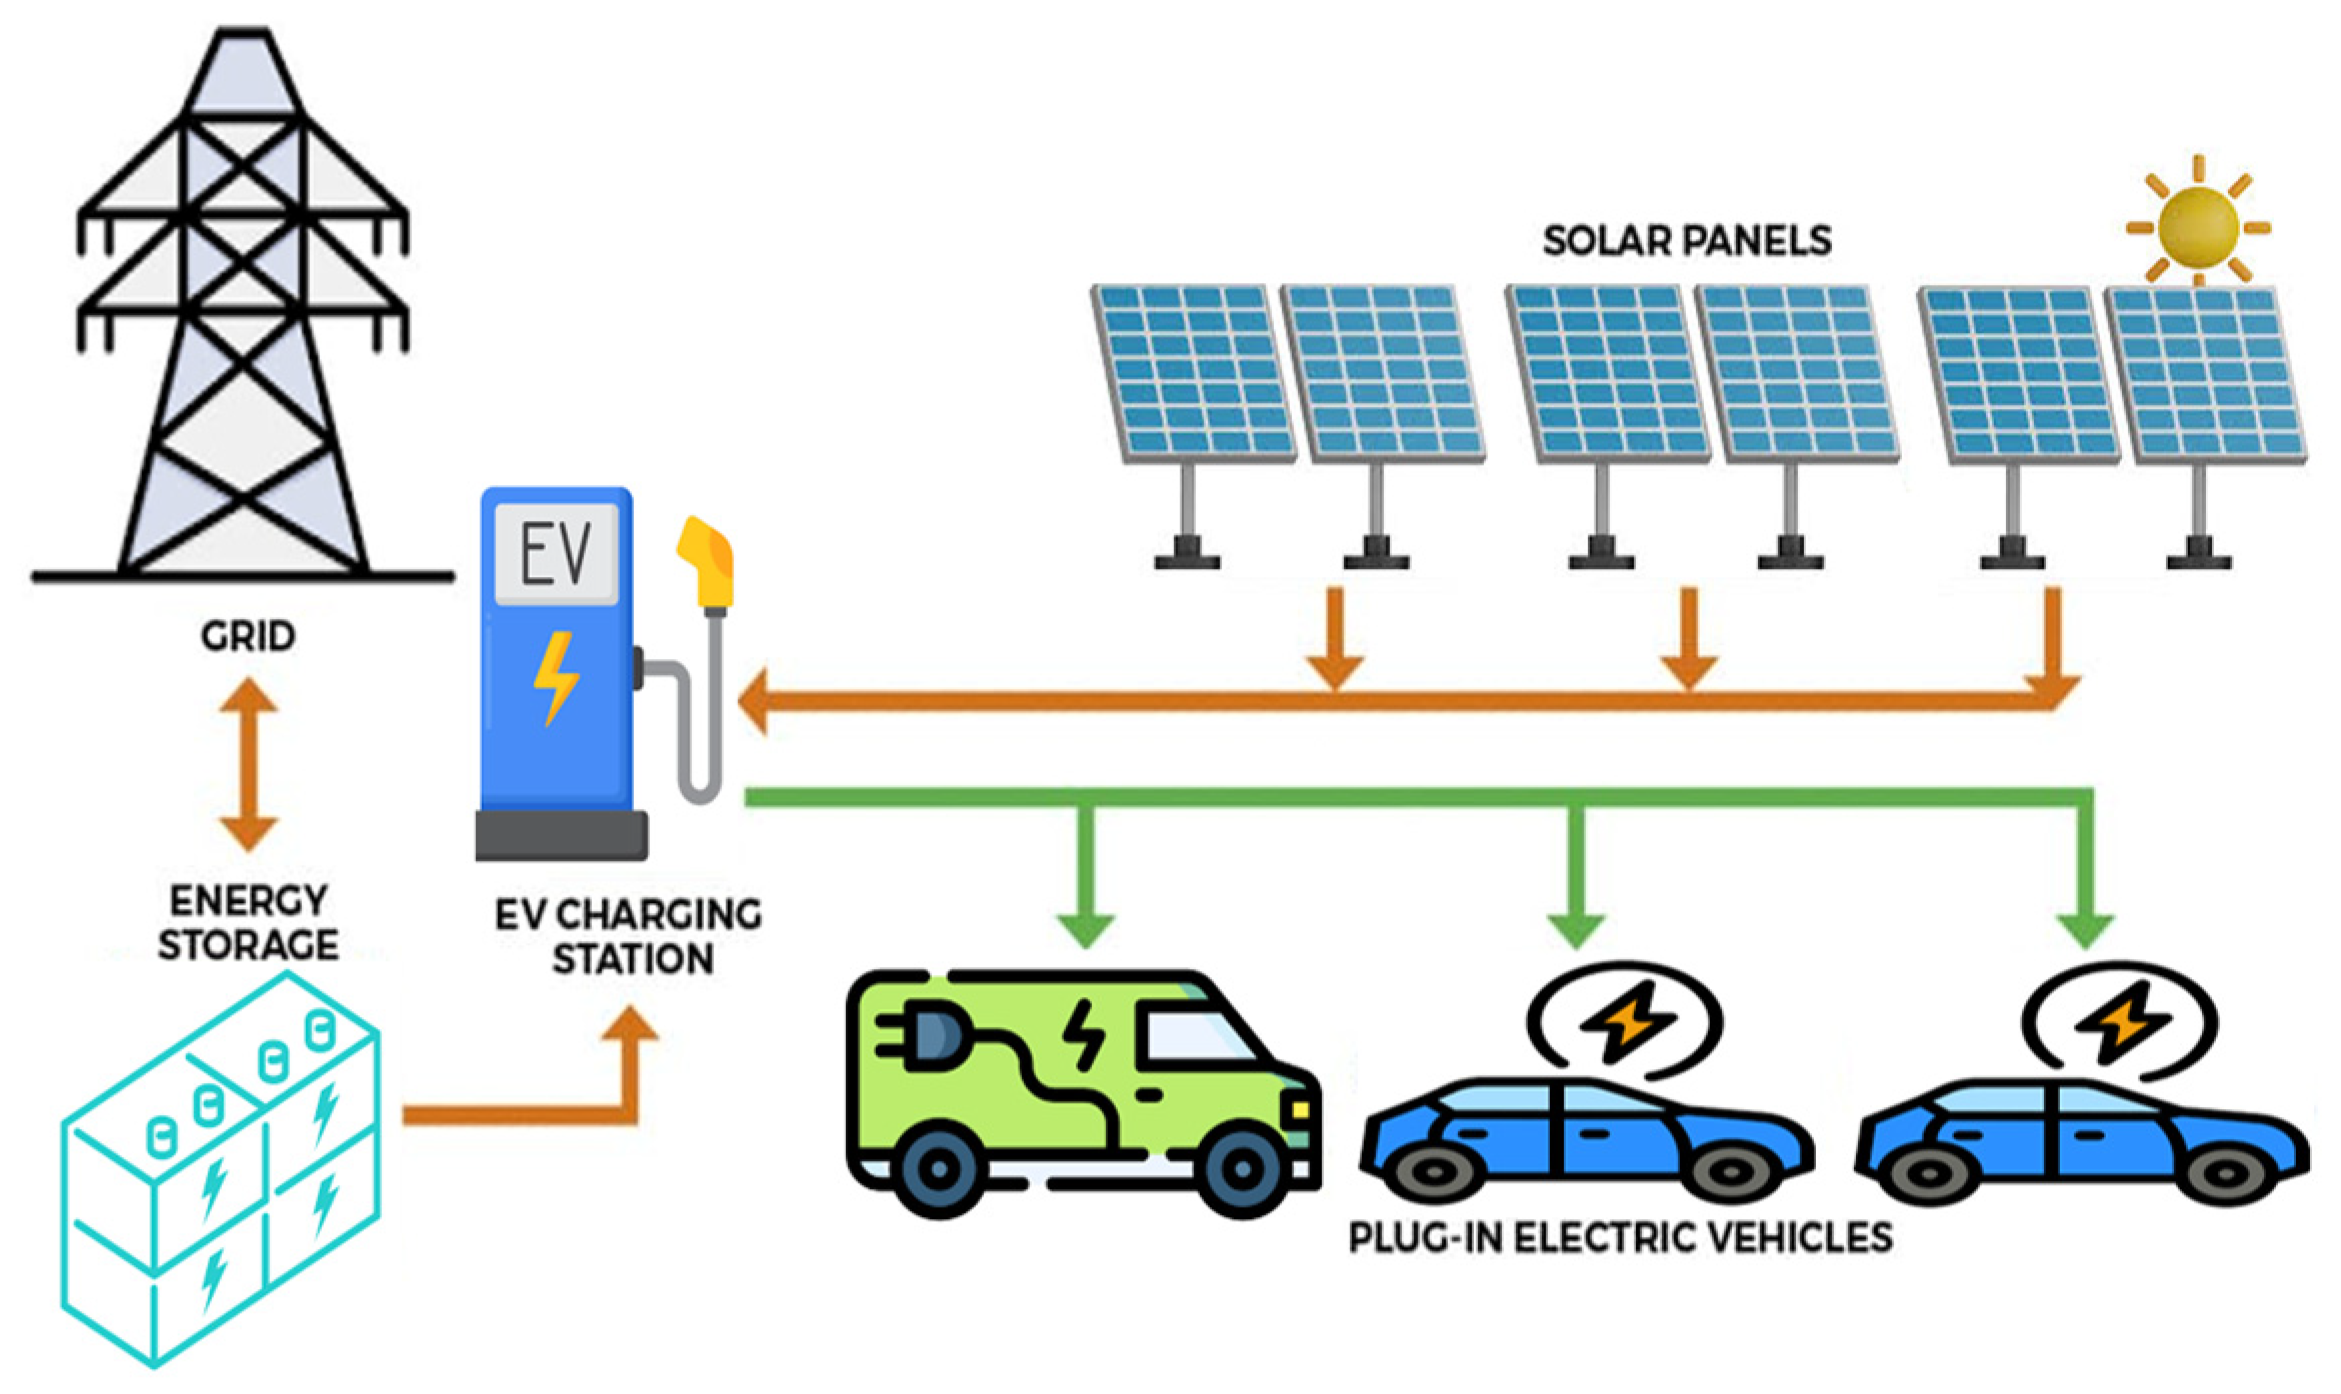
\includegraphics[width=0.7\textwidth]{Images/EVCI_diagram.png}
    \caption{\textbf{A typical EV charging infrastructure}~\cite{Deeum2023} \\Including electricity grid, 
    renewable generation (solar panels), energy storage systems, charging stations, 
    and plug-in electric vehicles. This integrated system highlights the importance of 
    coordinating generation, storage, and charging to ensure reliable and sustainable 
    operation.}
    \label{fig:EVCI_diagram}
\end{figure}

Emerging solutions aim to overcome these challenges. Dynamic charging, for 
instance, enables wireless on-road power transfer and has shown potential to 
reduce detours and charging time compared to conventional stations, though 
infrastructure costs remain high~\cite{Nguyen2024}. At the same time, digital twin 
technology is increasingly viewed as a powerful tool to manage the complexity 
of charging networks, enabling real-time monitoring, scenario analysis, and 
integration with renewable power and storage systems~\cite{Yu2024}. Such 
innovations highlight the importance of linking physical deployment with digital 
management systems to ensure reliability, sustainability, and scalability.

In summary, while EV adoption continues to expand rapidly, the success of the 
transition is inseparable from charging infrastructure. Planning, optimization, and 
digitalisation of charging networks will determine whether electrified transport 
can scale sustainably and equitably.

\subsection{Digital Twin and Simulation}

The increasing complexity of electric vehicle (EV) charging networks, 
their tight coupling with the power grid, and the variability of user 
behaviour make planning and operation challenging. Digital twin 
technology has emerged as a powerful approach to address these 
issues. A digital twin is defined as a ``live digital coupling of the state 
of a physical asset or process with a virtual representation that 
produces functional output''~\cite{Somers2023}. Unlike conventional 
models or static simulations, digital twins establish a continuous 
bi-directional link between the physical system and its digital replica, 
enabling real-time monitoring, predictive analytics, and feedback 
control~\cite{Liu2021Review,Enders2019}.

In the context of EV charging infrastructure, digital twins offer 
several advantages. First, they enable multi-scale simulation of 
charging demand and grid interaction, supporting optimal siting and 
sizing of charging stations. Second, they allow scenario analysis under 
uncertainty, including stochastic EV arrivals and variable renewable 
generation, thereby enhancing grid stability and resilience~\cite{Talusan2024}. 
Third, digital twins provide a platform for testing cyber-physical 
interactions, including cybersecurity assessment, without disrupting 
operational systems~\cite{Eckhart2019}. These capabilities make digital 
twin frameworks particularly suitable for managing charging networks 
within smart cities and integrating them into future vehicle-to-grid (V2G) 
and vehicle-to-building (V2B) systems.

\begin{figure}[ht!]
    \centering
    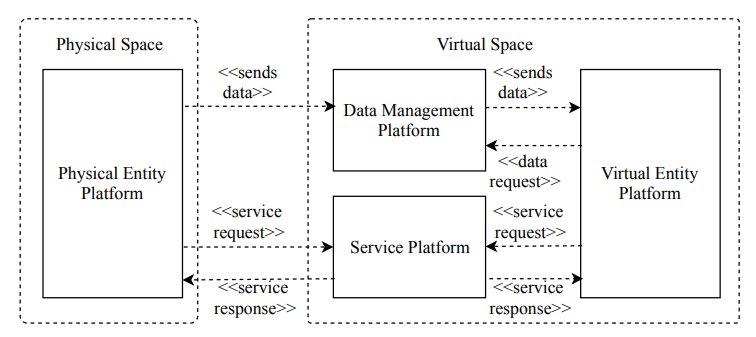
\includegraphics[width=0.7\textwidth]{Images/DT_diagram.png}
    \caption{\textbf{A Typical Digital Twin Framework}~\cite{8823809} \\
    The entities comprising the Physical Entity Platform send
specific data to the Data Management Platform. On request,
this platform sends data to the Virtual Entity Platform. The
Virtual Entity Platform can request concrete services from the
Service Platform and it receives back concrete information.
Furthermore, the underlying Physical Nodes of the Physical
Entity Platform can also send a service request to the Service
Platform and receive an appropriate response.
}
    \label{fig:DT_diagram}
\end{figure}


Simulation remains at the core of digital twin applications. Studies 
classify applications into \emph{simulation}, \emph{monitoring}, and 
\emph{control} purposes~\cite{Enders2019}. For EV charging, simulation 
provides the foundation to evaluate control strategies, optimize energy 
flows, and quantify environmental impacts. Discrete-event simulation 
platforms, such as OPTIMUS, extend these capabilities by integrating 
building energy use, grid events, and charging policies, allowing 
benchmarking of control algorithms under realistic conditions~\cite{Talusan2024}. 

In summary, digital twins bridge physical EV charging infrastructure 
with advanced simulation environments, enabling not only better 
operational decision-making but also long-term strategic planning. 
Their role as predictive, adaptive, and testable cyber-physical 
representations underscores their potential in achieving sustainable, 
resilient, and user-centric charging ecosystems.

\subsection{Data Models and Interoperability in Digital Twins}

Digital twins function as high-fidelity virtual counterparts of physical systems, supporting real-time monitoring, simulation, and control. However, realizing their full potential hinges on seamless data interoperability—the ability of multiple systems to exchange, interpret, and act upon shared information. Without standardized representations, digital twin implementations often remain siloed, each relying on proprietary formats that limit aggregation and coordinated analysis across domains~\cite{David2024}. Addressing this fragmentation requires robust standards and transformation mechanisms to align heterogeneous digital twin models, such as the Digital Twin Definition Language (DTDL) and the Asset Administration Shell (AAS)~\cite{Schmidt2023}.

Data models and ontologies play a crucial role in enabling interoperability. They provide a shared vocabulary and structure that allow systems to interpret information consistently across semantics, constraints, and behaviors~\cite{Karabulut2023}. Semantic technologies, knowledge graphs, and ontology-based integration frameworks are increasingly used to bridge modeling languages and domains, facilitating automated data fusion and richer collaboration between digital twins~\cite{Dunbar2022}. In addition, conceptual interoperability frameworks, such as those proposed by the Digital Twin Consortium, define atomic data entities and standardized messaging patterns to support modular composition of digital twins across system boundaries~\cite{Budiardjo2021}.

For infrastructures such as electric vehicle (EV) charging networks, interoperable data models are indispensable. They enable cross-system coordination between charging stations, grid services, and building energy systems; support automated integration of sensor data, user behavior, and energy flows; and provide a foundation for composable architectures where charging, storage, and renewable generation twins can interact within a unified ecosystem. Ensuring accurate, semantic-level interoperability is thus a prerequisite for building comprehensive, reliable, and scalable digital twin systems that can address the challenges of sustainable and intelligent mobility.


% \section{Inclure des images}



% \begin{figure}[ht!]
%     \centering
%     \includegraphics[width=0.35\textwidth]{example-image-a}
%     \includegraphics[width=0.35\textwidth]{example-image-b}
%     \caption{\textbf{Titre.} \lipsum[1][1-5]}
%     \label{fig:image2}
% \end{figure}



% \section{Listes et tableaux}

% \textbf{Insérer une liste~:}
% \begin{itemize}
%     \item Premier niveau
%     \begin{itemize}
%         \item[(i)] Deuxième niveau
%         \item[(ii)] Un autre élément au deuxième niveau
%     \end{itemize}
%     \item Un autre élément au premier niveau
%         \begin{itemize}
%         \item[(a)] Deuxième niveau
%         \item[(b)] Un autre élément au deuxième niveau
%     \end{itemize}
% \end{itemize}
% \bigskip

% \textbf{Insérer un tableau simple~:} 
% \begin{table}[H]
%     \centering
%     \begin{tabular}{|c|c|c|c|c|c|c|c|c|c|}
%         \hline
%         A & B & C & D & E & F & G & H & I & \dots \\
%         \hline
%         1 & 2 & 3 & 4 & 5 & 6 & 7 & 8 & 9 & \dots\\
%         10 & 11 & 12 & 13 & 14 & 15 & 16 & 17 & 18 & \dots \\
%         \hline
%     \end{tabular}
%     \caption{\textbf{Titre.} \lipsum[1][1-3]}
%     \label{tab:table-label}
% \end{table}

% \textbf{Autre style de tableau~:} 
% \begin{table}[H]
%     \centering
%     \begin{tabular}{c c c c c}
%         \hline
%         \textbf{Col1} & \textbf{Col2} & \textbf{Col3} & \textbf{Col4} & \textbf{Col5} \\
%         \hline
%         1 & 2 & 3 & 4 & 5 \\
%         1 & 2 & 3 & 4 & 5 \\
%         \hline
%     \end{tabular}
%     \caption{\textbf{Titre.} \lipsum[1][1-3]}
%     \label{tab:table-label}
% \end{table}


% \section{Insertion de code Python}
% \textbf{Insérer du code en \textit{inline}~:} \texttt{print("Hello, World!")}.\\


% \textbf{Insérer du code en \textit{inline} avec coloration syntaxique~:} \mintinline{python}{print("Hello, World!")}.\\

% \textbf{Insérer du code en bloc avec coloration syntaxique~:} 
% \begin{minted}[bgcolor=codebg,fontsize=\small,frame=lines,linenos]{python}
% def factorial(n):
%     if n == 0:
%         return 1
%     else:
%         return n * factorial(n - 1)

% # Example usage
% print(factorial(5))  # Output: 120
% \end{minted}



% \section{Expressions mathématiques}
% \subsection{Théorèmes, propositions, définitions, lemmes, demonstrations...}

% \begin{theorem}
%     \lipsum[1][1-4]
% \end{theorem}

% \begin{proof}
%     \lipsum[1][1-4]
% \end{proof}

% \begin{proposition}
%     \lipsum[1][1-4]
% \end{proposition}

% \begin{definition}
%     \lipsum[1][1-4]
% \end{definition}

% \begin{remark}
%     \lipsum[1][1-4]
% \end{remark}

% \begin{lemma}
%     \lipsum[1][1-4]
% \end{lemma}


% \subsection{Equations et calculs sur plusieurs lignes}

% \subsubsection*{Une simple équation}
% \begin{equation}
%     e = mc^2
% \end{equation}

% \subsubsection*{Une équation sur plusieurs lignes}
% \begin{equation}
%     \begin{split}
%         \mathbb{E}(aX + Y) &= \mathbb{E}(aX) + Y\\
%                            &= a\mathbb{E}(X) + Y
%     \end{split}
% \end{equation}

% \subsubsection*{Une équation avec plusieurs cas}
% \begin{equation}
%     u_n =
%     \begin{cases}
%         1 \text{ if } n\equiv0 \mod 2\\
%         0 \text{ if } n\equiv1 \mod 2 \\
%     \end{cases}
% \end{equation}

% \subsubsection*{Insérer une série de calculs}
% \begin{align*}
%     x &= 0.999\ldots \\
%     10x &= 9.999\ldots \\
%     10x - x &= 9.999\ldots - 0.999\ldots \\
%     9x &= 9 \\
%     x &= 1 \\
%     0.999\ldots &= 1
% \end{align*}

% \subsection{Utilisation du glossaire}

% \newglossaryentry{esperance}{
%     name=espérance,
%     description={Valeur moyenne théorique d'une variable aléatoire}
% }


% Référence au glossaire : \gls{esperance}.  




